\section{Sensitivity and Counterfactual Scenarios}
\label{sec:sensitivity}
A model becomes easier to interpret when its conclusions are tested against changes in its assumptions. We use sensitivity analysis to ask which resource would matter next if one cost were reduced. These are counterfactual scenarios. They do not represent overclocking experiments, measurements on multiple devices, or estimates of future hardware capabilities.

\subsection{Bandwidth sweep}
Figure~\ref{fig:bandwidth} fixes $N=8192$ and $d=64$ while varying the hypothetical bandwidth. The materialized schedule initially benefits from increasing this parameter because transfer is its active component. Once arithmetic dominates, the curve flattens. The tiled schedule can reach that region earlier because its modeled byte count is smaller. The resulting speedup is therefore not constant across hypothetical devices.

\begin{figure}[t]
 \centering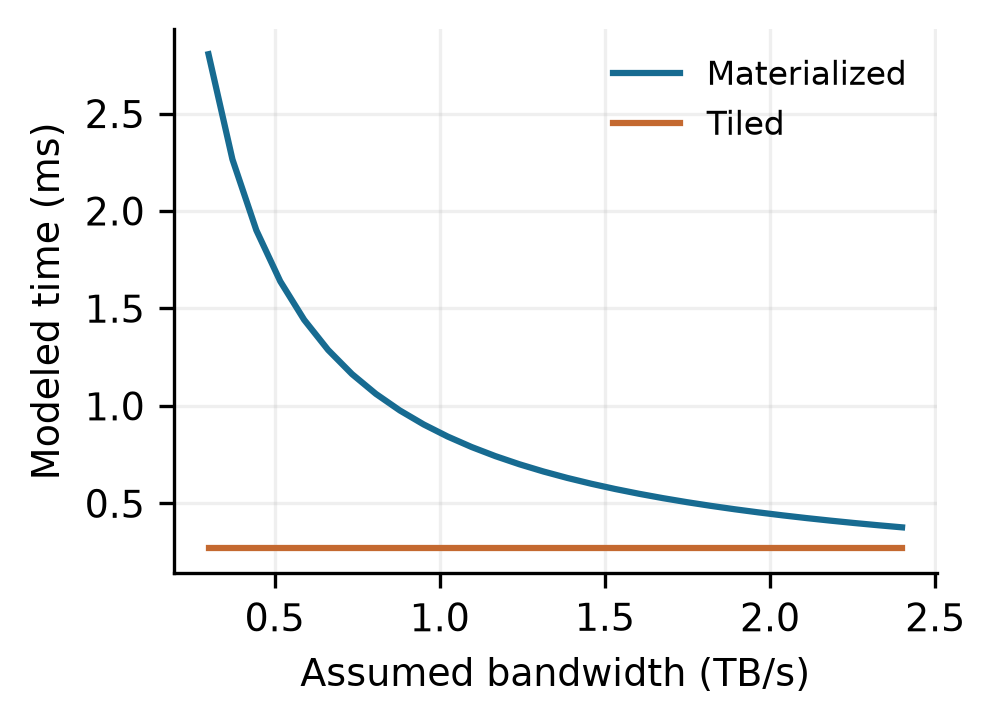
\includegraphics[width=\linewidth]{assets/bandwidth.png}
 \caption{Synthetic bandwidth counterfactual at $N=8192,d=64$. All other assumptions are held fixed. The flat region is a model constraint, not a measured saturation point.}
 \label{fig:bandwidth}
\end{figure}

The crossover has an operational interpretation. If a profiler shows that an implementation is already limited by arithmetic or dependency chains, optimizing a transfer that is fully hidden may not improve elapsed time. Conversely, a reduction in traffic can still improve energy or shared-resource interference, neither of which is represented here. A flat time curve is therefore not evidence that the removed bytes are useless in every system objective; it says that this objective and this model do not value them at that point.

\subsection{Arithmetic efficiency}
Figure~\ref{fig:efficiency} varies the arithmetic fraction while keeping nominal peak throughput fixed. The tiled schedule is more sensitive over the region where arithmetic limits it. This supports a sequential way of thinking about optimization: reducing one bottleneck can expose another. It does not justify assuming that the effective fraction can be raised independently in a real kernel, because occupancy, synchronization, and instruction mix may be coupled.

\begin{figure}[t]
 \centering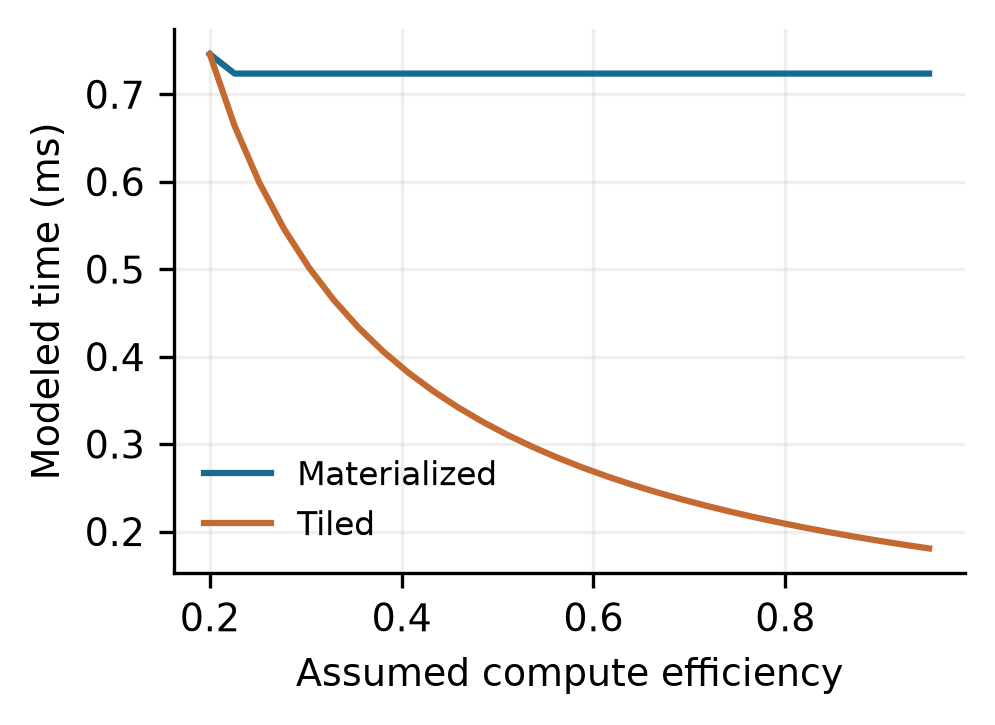
\includegraphics[width=\linewidth]{assets/efficiency.png}
 \caption{Synthetic arithmetic-efficiency sweep. The horizontal axis is an assumed effective fraction of peak, not a reported utilization measurement.}
 \label{fig:efficiency}
\end{figure}

Work-partitioning research makes the distinction between fewer transfers and better execution efficiency particularly relevant~\cite{dao2023flashattention2}. Our model retains only a scalar efficiency parameter, so it cannot distinguish between reasons for low efficiency. Different causes may require opposite implementation changes. A larger tile may improve reuse but increase register demand; more parallel tasks may improve occupancy but require additional synchronization. The scalar is useful for sensitivity, not for diagnosing a kernel.

\subsection{Launch overhead and small workloads}
The launch term bounds the improvement obtainable by changing the resource terms. If both schedules have nearly identical fixed overhead, reducing a small variable cost cannot make the whole operation arbitrarily faster. This behavior is visible in the left side of Figure~\ref{fig:time}. The model does not include fusion across attention and neighboring operators, so it also does not estimate how a different integration boundary would change that overhead.

A future empirical study should report its timing boundary precisely. Host dispatch, device synchronization, graph replay, and batch formation can produce different notions of latency. An author should not compare a device-only timing for one implementation with an end-to-end timing for another. The correct boundary depends on the research question, but it must remain consistent within a comparison.

\subsection{End-to-end limits}
Let $f$ be the fraction of an application's baseline time spent in the modeled attention operation and let $S$ be its local speedup. If everything else is unchanged, the corresponding end-to-end ratio is
\begin{equation}
 S_{\mathrm{end}}=\frac{1}{(1-f)+f/S}.
 \label{eq:end}
\end{equation}
This equation is an accounting identity under the stated decomposition. It does not imply that $f$ is constant when batch size, memory pressure, or scheduling changes. Those interactions can be important, but they require additional evidence rather than an unqualified extrapolation from a kernel result.

For illustration, a local ratio of three and a baseline attention share of one half produce an end-to-end ratio of 1.5. With a share of one fifth, the ratio is only about 1.15. These arithmetic examples are not application measurements. They show why a paper should disclose the attention share before presenting a local improvement as an overall system benefit.
